\documentclass[a4paper,man,floatsintext,longtable,noextraspace,10pt]{apa6}

\usepackage[english]{babel}
\usepackage[utf8x]{inputenc}
\usepackage{amsmath}
\usepackage{graphicx}
\usepackage[colorinlistoftodos]{todonotes}
\usepackage{hyperref}

\usepackage{booktabs}
\usepackage{longtable}
\usepackage{array}
\usepackage{multirow}
\usepackage{wrapfig}
\usepackage{float}
\usepackage{colortbl}
\usepackage{pdflscape}
\usepackage{tabu}
\usepackage{threeparttable}
\usepackage{threeparttablex}
\usepackage[normalem]{ulem}
\usepackage{makecell}
\usepackage{xcolor}
% make captions italic

% number lines
% \usepackage{lineno}
% \linenumbers
            
% definitions for citeproc citations
\NewDocumentCommand\citeproctext{}{}
\NewDocumentCommand\citeproc{mm}{%
\begingroup\def\citeproctext{#2}\cite{#1}\endgroup}
\makeatletter
% allow citations to break across lines
\let\@cite@ofmt\@firstofone
% avoid brackets around text for \cite:
\def\@biblabel#1{}
\def\@cite#1#2{{#1\if@tempswa , #2\fi}}
\makeatother
\newlength{\cslhangindent}
\setlength{\cslhangindent}{1.5em}
\newlength{\csllabelwidth}
\setlength{\csllabelwidth}{3em}
\newenvironment{CSLReferences}[2] % #1 hanging-indent, #2 entry-spacing
{\begin{list}{}{%
  \setlength{\itemindent}{0pt}
  \setlength{\leftmargin}{0pt}
  \setlength{\parsep}{0pt}
  % turn on hanging indent if param 1 is 1
  \ifodd #1
  \setlength{\leftmargin}{\cslhangindent}
  \setlength{\itemindent}{-1\cslhangindent}
  \fi
  % set entry spacing
  \setlength{\itemsep}{#2\baselineskip}}}
{\end{list}}
\usepackage{calc}
\newcommand{\CSLBlock}[1]{\hfill\break\parbox[t]{\linewidth}{\strut\ignorespaces#1\strut}}
\newcommand{\CSLLeftMargin}[1]{\parbox[t]{\csllabelwidth}{\strut#1\strut}}
\newcommand{\CSLRightInline}[1]{\parbox[t]{\linewidth - \csllabelwidth}{\strut#1\strut}}
\newcommand{\CSLIndent}[1]{\hspace{\cslhangindent}#1}

% tightlist
\providecommand{\tightlist}{%
  \setlength{\itemsep}{0pt}\setlength{\parskip}{0pt}}

\shorttitle{}

% flow chart
\usepackage{tikz}
\usetikzlibrary{shapes.geometric, arrows, positioning, calc, shapes.multipart}

% Custom styles for the flowchart
\tikzstyle{datasource} = [rectangle, rounded corners, minimum width=2.5cm, minimum height=1cm,text centered, draw=blue!60, fill=blue!5]
\tikzstyle{process} = [rectangle, minimum width=3cm, minimum height=1cm, text centered, draw=green!60, fill=green!5]
\tikzstyle{decision} = [diamond, minimum width=3cm, minimum height=1cm, text centered, draw=red!60, fill=red!5]
\tikzstyle{arrow} = [thick,->,>=stealth]
\tikzstyle{output} = [rectangle, rounded corners, minimum width=3cm, minimum height=1cm, text centered, draw=purple!60, fill=purple!5]

\setlength\parindent{1.27cm}

\begin{document}
\thispagestyle{otherpage}

%\maketitle

% Change \title, \date, remove \author:
\begin{large}
\textbf{Replication: Hybrid Open Access in Transformative Agreements}
\end{large}

% Add below \maketitle:
\newcommand{\orcid}{%
  \begingroup\normalfont
  
\includegraphics[height=0.9em]{orcid_logo}% removed .png extension
  \endgroup
}

Najko Jahn\textsuperscript{1}\textsuperscript{*} 
(\orcid{} \href{https://orcid.org/0000-0001-5105-1463}{\color{black}{0000-0001-5105-1463}})

\textsuperscript{1} Göttingen State and University Library, University of Göttingen, Germany. \\

\textsuperscript{*} Correspondence: \href{mailto:najko.jahn@sub.uni-goettingen.de}{\color{black}{najko.jahn@sub.uni-goettingen.de}} 

\section*{Abstract}
{}
{\textbf{Keywords}: hybrid open access, transformative agreements, scholarly publishing, big deals, bibliometrics}

\newpage

% QSS wants numbered sections
\setcounter{secnumdepth}{2}

\section{Introduction}\label{introduction}

This study aims to demonstrate the suitability of open scholarly data
sources for assessing the impact of transformative agreements on hybrid
open access. To achieve this, a replication study was conducted by
comparing results from hoaddata, an openly available and continuously
updated dataset on hybrid open access uptake based on Crossref,
OpenAlex, and the cOAlition S Journal Checker Tool, with the established
bibliometric databases Web of Science and Scopus.

This study focuses on the coverage of hybrid journal portfolios included
in transformative agreements between 2019 and 2023. Special attention is
given to potential differences in open access uptake by country when
comparing first-author affiliation data to corresponding authorships.
This is crucial because the lack of publicly available invoicing data
corresponding to authorships plays an essential role in determining
whether an open-access article is supported through transformative
agreements. Data on corresponding authorships have been available on the
Web of Science and Scopus for much longer than in open databases such as
OpenAlex, where this information is still being roled out at the time of
writing. Because of this weakness, open approaches such as hoaddata and
related research use first-authorship data instead.

By conducting a large-scale comparative analysis, this study aims to

\begin{enumerate}
\def\labelenumi{\arabic{enumi}.}
\tightlist
\item
  Determine the strengths and weaknesses of using open data sources in
  monitoring the impact of transformative agreements on hybrid open
  access publishing.
\item
  Assess the coverage and accuracy of open data sources compared with
  established bibliometric databases.
\item
  Evaluate the reliability of first author affiliation data as a proxy
  for corresponding authorship in the context of open access uptake
  analysis.
\end{enumerate}

\section{Background -- Evidence base to measure the effects of
transformative
agreements}\label{background-evidence-base-to-measure-the-effects-of-transformative-agreements}

\subsection{Anforderungen an das
Monitoring}\label{anforderungen-an-das-monitoring}

\begin{itemize}
\tightlist
\item
  esac guidelines
\item
  gemeinsamkeiten und unterschiede zu apc (listenpreise, tatsächliche
  zahlungen, zentrales invoicing, rabatte, waivers)
\item
  insitutionen covern cas, jedoch kann es zu unterschiedlichen
  verrechnugnsformen führen (antielig mit förderer, splitting
  innerhaklbd er einrichtung)
\end{itemize}

\subsection{Bibliometrische Evidenzen}\label{bibliometrische-evidenzen}

\begin{itemize}
\tightlist
\item
  allgmeeiner uptake
\item
  wachstum apcs
\item
  wachstum verträge (konsortien, forschung)
\item
  konsequenzen
\end{itemize}

\section{Data and methods}\label{data-and-methods}

This study aims to demonstrate the suitability of open scholarly data
sources for assessing the impact of transformative agreements on hybrid
open access. As shown in Figure \ref{fig:workflow}, the methodology
involved comparing hoaddata, an openly available collection of open
research information on hybrid open access, with the bibliometric
databases Web of Science and Scopus. This section introduces the initial
data sources followed by a presentation of the necessary pre-processing
steps to obtain eligible articles from transformative agreements by
using author roles (first and corresponding) and harmonised affiliation
data.

\begin{figure}[htbp]
\centering
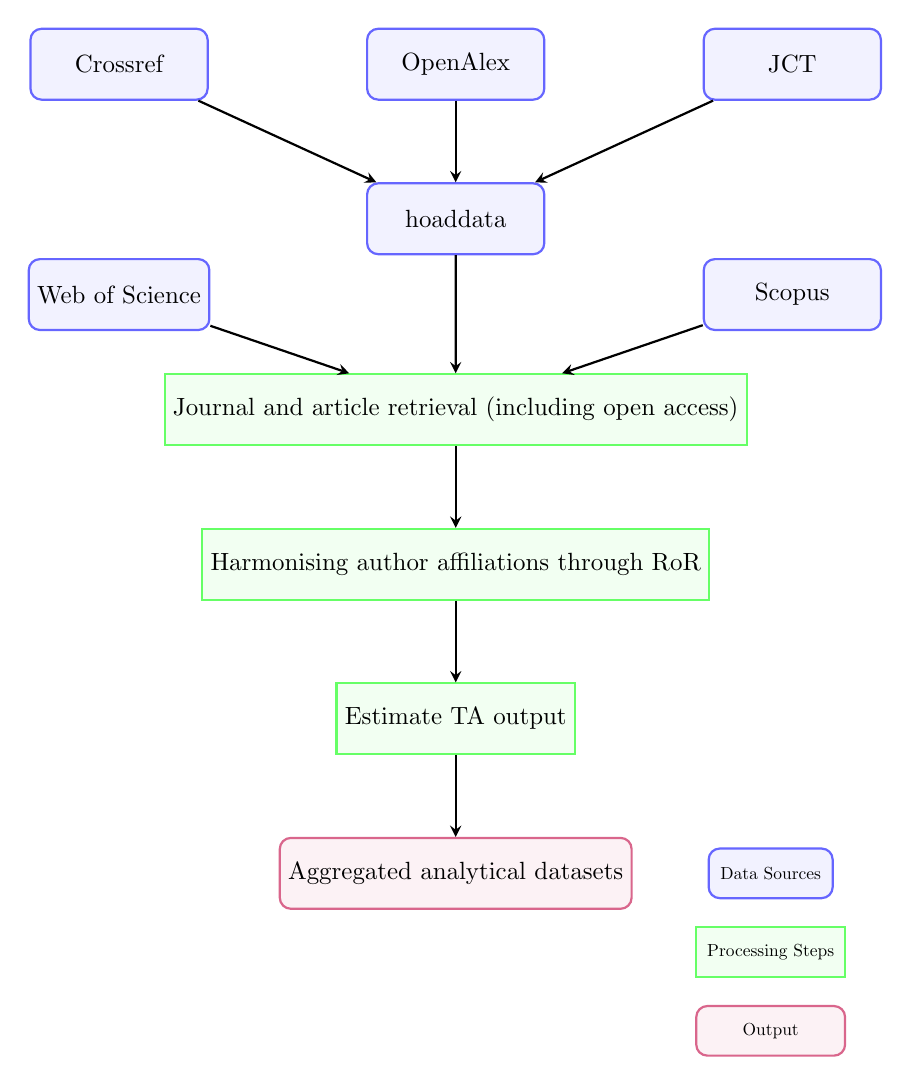
\begin{tikzpicture}[node distance=2cm, thick,scale=1, every node/.style={scale=0.9}]    
% Data Sources
    \node (crossref) [datasource] {Crossref};
    \node (openAlex) [datasource, right=of crossref] {OpenAlex};
    \node (jct) [datasource, right=of openAlex] {JCT};
    \node (wos) [datasource, below=of crossref] {Web of Science};
    \node (scopus) [datasource, below=of jct] {Scopus};
    
    % Processing Steps
    \node (hoaddata) [datasource, below=1.5cm of $(crossref)!1!(openAlex)$] {hoaddata};
    \node (kb) [process, below=1cm of $(wos)!0.5!(scopus)$] {Journal and article retrieval (including open access)};
    
 % Matching Process - Fixed line break syntax
    \node (matching) [process, below=1.5cm of $(hoaddata)!1!(kb)$] {Harmonising author affiliations through RoR};

 % Aggregation
    \node (transmatch) [process, below=1.5cm of $(matching)!1!(matching)$] {Estimate TA output};
        
    % Output
    \node (analysis) [output, below=1.5cm of $(transmatch)!1!(transmatch)$] {Aggregated analytical datasets};
    
    % Arrows
    \draw [arrow] (crossref) -- (hoaddata);
    \draw [arrow] (openAlex) -- (hoaddata);
    \draw [arrow] (jct) -- (hoaddata);
    \draw [arrow] (hoaddata) -- (kb);
    \draw [arrow] (wos) -- (kb);
    \draw [arrow] (scopus) -- (kb);
    \draw [arrow] (kb) -- (matching);
    \draw [arrow] (matching) -- (transmatch);
    \draw [arrow] (transmatch) -- (analysis);

    
    % Legend
    \node [datasource, scale=0.7] at ($(analysis)+(4,0)$) {Data Sources};
    \node [process, scale=0.7] at ($(analysis)+(4,-1)$) {Processing Steps};
    \node [output, scale=0.7] at ($(analysis)+(4,-2)$) {Output};
\end{tikzpicture}
\caption{Data processing workflow for comparing hybrid open access uptake across bibliometric data sources. The workflow shows how data from different sources (Crossref, OpenAlex, JCT, Web of Science, and Scopus) is processed and matched using ROR identifiers to enable comparative analysis. TA = Transformative Agreement}
\label{fig:workflow}
\end{figure}

\subsection{Data sources}\label{data-sources}

\subsubsection{hoaddata}\label{hoaddata}

hoaddata, developed and maintained by the author to support open access
monitoring and research (Jahn, 2025), is an R data package comprising
information about the uptake of hybrid open access since 2017 collected
from several openly available data sources. It combines article-level
metadata from Crossref and OpenAlex with transformative agreement
information from the cOAlition S Journal Checker Tool (JCT), which links
journal and institutional data to agreements in the ESAC registry.

As discussed elsewhere (Jahn, 2025), hoaddata uses a unified dataset of
historic JCT snapshots since July 2021, which were enriched with ISSN
variants linked to an ISSN-L and associated ROR-IDs representing
university hospitals or institutes of large research organisations,
according to OpenAlex' institution entity. A comprehensive exclusion of
fully open access journals using multiple journal lists (DOAJ, OpenAlex,
Bielefeld) was performed to identify hybrid journals. hoaddata relies on
Crossref for obtaining journal publication volume and open access status
through Creative Commons licence information relative to the published
version (``version of record''). Because of limited affiliation metadata
in Crossref (Eck \& Waltman, 2022), hoaddata sources first-author
affiliations from OpenAlex.

hoaddata follows good practices for computational reproducibility using
R (Marwick et al., 2018). The package, which includes data, code, a test
suite and documentation, is openly available on GitHub. To ensure
computational reproducibility while aggregating the data, a GitHub
Actions continuous integration and delivery (CI/CD) workflow interfaces
with the SUB Göttingen's open scholarly data warehouse based on Google
BigQuery, which provides high-performant programmatic access to monthly
snapshots of Crossref and OpenAlex. The workflow has run regularly to
fetch updates from these data sources since 2022. The package version
used in this study is 0.3, containing data from the Crossref 2024-08
dump provided to Crossref Metadata Plus subscribers and the OpenAlex
2024-08-29 monthly dump. This version including the computation log is
available on GitHub
(https://github.com/subugoe/hoaddata/releases/tag/v.0.3).

\subsubsection{Web of Science}\label{web-of-science}

Clarivate Analytics' Web of Science (WoS) is a well-established
proprietary bibliometric database consisting of several collections
(Birkle et al., 2020). The collections considered in this study were the
Science Citation Index Expanded (SCIE), the Social Sciences Citation
Index (SSCI) and the Arts \& Humanities Citation Index (AHCI),
collectively referred to as Web of Science Primary (WoS Primary).

The WoS Primary provides important data points for analysing open
access: author affiliations and roles, differentiation of journal
articles into document types representing different types of journal
contributions, such as original articles or reviews, and open access
status information derived from OurResearch's Unpaywall, the same
provider as Openalex. However, it lacks information about journals and
articles under transformative agreements.

For programmatic access to article-level data, this study used the
database of the Kompetenznetzwerk Bibliometrie (KB) in Germany. The KB
processes raw XML data provided by Clarivate Analytics, which is
provided as an in-house PostgreSQL database under a uniform schema. To
support reproducibility, KB maintains annual snapshots of the database.
Accordingly, this study used the annual snapshot from April 2024
(wos\_b\_202404), which is considered to cover almost the entire
previous publication year (Schmidt et al., 2024).

\subsubsection{Scopus}\label{scopus}

Elsevier's Scopus, launched in 2004, is another widely used proprietary
bibliometric database for measuring research (Baas et al., 2020).
Similar to the Web of Science, Scopus is selective with regard to the
journals it indexes. However, its coverage is substantially more
extensive than that of the Web of Science collections considered in this
study (Singh et al., 2021; Visser et al., 2021). With detailed metadata
about article types, open access status information derived from
Unpaywall, author roles, and disambiguated affiliations, Scopus also
contains important data to assess open access uptake, although no direct
information regarding transformative agreements was available at the
time of the study.

This study used the Scopus annual snapshot of April 2024 as provided by
the KB (scp\_b\_202404). The same KB curation effort was applied to the
Scopus raw data as for the Web of Science (Schmidt et al., 2024).

\subsection{Data processing steps}\label{data-processing-steps}

\subsubsection{Determining hybrid journal publication
volume}\label{determining-hybrid-journal-publication-volume}

The hoaddata package (v.0.3) provided an enriched and unified list of
hybrid journals in transformative agreements according to the JCT,
covering agreements active from July 2021 to July 2024 according to the
ESAC registry.

Article metadata was retrieved from each databse using all ISSN variants
linked to an ISSN-L. The metadata included DOIs, publication dates,
article types, open access information as well as author roles and
institutional affiliations. Publication years were determined using the
earliest known date of publication in a journal. articles in hoaddata,
this corresponded to Crossref's issued date. For Web of Science and
Scopus, the earliest publication date was used where available, with
Scopus dates specifically determined by the KB through version tracking
of the raw data.

Many transformative agreements typically cover only certain types of
journal articles, in particular original research articles including
reviews. Because of limited information on these document types in open
scholarly data (Haupka et al., 2024), hoaddata used an extended version
of Unpaywall's paratext recognition approach to exclude non-scholarly
content (Piwowar et al., 2018). To exclude conference supplements, which
are also often not covered by transformative agreements, only articles
published in regular issues, indicated by numerical pagination, were
considered. For Web of Science and Scopus, their established document
type classifications were used to identify original research articles
and reviews, referred to as core articles throughout this study.

\subsubsection{Identifying open access articles in hybrid
journals}\label{identifying-open-access-articles-in-hybrid-journals}

Published articles were considered hybrid open access when they were
made freely available under a Creative Commons license on publishers'
platforms. While hoaddata sourced this information from Crossref license
metadata, Web of Science and Scopus relied on Unpaywall. Unpaywall
supplements Crossref metadata by parsing publisher websites directly,
addressing cases where publishers do not provide machine-readable
Creative Commons license information (Piwowar et al., 2018). This
additional parsing remains necessary despite transformative agreement
workflows requiring license information during DOI registration
(Geschuhn \& Stone, 2017). Both Web of Science and Scopus defined hybrid
open access consistently as content available under Creative Commons
licenses on publisher platforms, distinguishing it from bronze open
access that lack such explicit license information.

\subsubsection{Harmonising author affiliations across
databases}\label{harmonising-author-affiliations-across-databases}

Author affiliations were retrieved for both first and, if available,
corresponding authors across all databases to prepare the linking
between articles and institutions covered by transformative agreements.
To handle different address variants, database-specific affiliation
identifiers were used: ROR-IDs from OpenAlex for hoaddata, affiliation
enhanced names for Web of Science, and Scopus Affiliation Identifiers
for Scopus. Additionally, ISO country codes were retrieved for each
author's address to compile country-level statistics. These country
codes for Web of Science and Scopus were provided by the KB.

Because neither Web of Science nor Scopus support ROR IDs---the
institution identifier used by the JCT---a two-step matching process was
implemented to harmonise affiliation data. First, 2,782,540 articles
from 6,457 institutions with ROR-IDs in the JCT data since 2017
(according to hoaddata) were processed to map first authors' ROR-IDs to
corresponding proprietary affiliation identifier in Web of Science and
Scopus using DOI matching. Then, an algorithm selected the most frequent
ROR ID and proprietary identifier pairs to handle multiple affiliations
and organisational hierarchy differences.

This process linked 6,375 ROR IDs to 4,894 Scopus Affiliation IDs, and
6,034 ROR IDs to 4,894 enhanced affiliation strings in the Web of
Science. Quality evaluation through random sampling of 50 pairs revealed
an error rate of 22\% for Web of Science (11 mismatches) and 6\% for
Scopus (3 mismatches). Upon inspection, these mismatches primarily
occurred with less-represented institutions having only a few
publications, introduced through multiple affiliations of single
authors. The difference between databases suggests that Scopus's
affiliation control aligns more closely with ROR than that of the Web of
Science.

\subsubsection{Estimating open access in hybrid journals covered by
transformative
agreements}\label{estimating-open-access-in-hybrid-journals-covered-by-transformative-agreements}

Based on these matching tables, articles eligible under transformative
agreements could also be retrieved from Web of Science and Scopus,
although they did not contain the ROR IDs used by the JCT. The
estimation of eligible articles followed Jahn (2025) and included a
matching of both journals and participating institutions according to
the Transformative Agreement Data dump for each of the data sources
examined. The matching also took into account the duration of agreements
according to the ESAC registry, with only those matches where an
agreement was actually in place being considered for subsequent
analysis.

\subsection{Data records}\label{data-records}

As a result of the comprehensive data processing described above,
datasets on open access in hybrid journals included in transformative
agreements were aggregated for each database at country and journal
level by year. Table~\ref{tbl-methods_overview_tab} provides a general
overview of the coverage between 2019 and 2023 per database. It shows
that the majority of hybrid journals published at least one original
research article or review marked as core during the five-year period.
These journals formed the basis for the subsequent aggregation of
publication metrics.

\begin{table}

\caption{\label{tbl-methods_overview_tab}Coverage of hybrid journals in
transformative agreements 2019-23.}

\centering{

\centering
\begin{tabular}[t]{lrrr}
\toprule
\textbf{} & \textbf{HOAD} & \textbf{Web of Science} & \textbf{Scopus}\\
\midrule
\addlinespace[0.3em]
\multicolumn{4}{l}{\textbf{Hybrid journal metrics}}\\
\hspace{1em}Active journals & 12,890 & 8,655 & 11,888\\
\hspace{1em}Active journals (core) & 12,888 & 8,655 & 11,878\\
\hspace{1em}Active journals (core) with OA & 11,348 & 8,392 & 11,313\\
\addlinespace[0.3em]
\multicolumn{4}{l}{\textbf{Publication metrics}}\\
\hspace{1em}Total published articles & 9,740,015 & 8,616,053 & 8,117,644\\
\hspace{1em}Core articles & 8,158,425 & 6,708,083 & 7,317,703\\
\addlinespace[0.3em]
\multicolumn{4}{l}{\textbf{Digital Object Identifier (DOI) coverage}}\\
\hspace{1em}Articles with DOI & 9,740,015 & 7,713,796 & 8,105,112\\
\hspace{1em}Core articles with DOI & 8,158,425 & 6,695,661 & 7,314,327\\
\addlinespace[0.3em]
\multicolumn{4}{l}{\textbf{Open Access (OA) metrics}}\\
\hspace{1em}OA articles & 998,699 & 1,112,758 & 974,099\\
\hspace{1em}Core OA articles & 969,817 & 1,019,784 & 922,578\\
\addlinespace[0.3em]
\multicolumn{4}{l}{\textbf{Core articles with affiliation data}}\\
\hspace{1em}First author articles & 7,242,542 & 6,294,855 & 7,232,017\\
\hspace{1em}Corresponding author articles & 5,534,207 & 6,291,441 & 6,898,487\\
\bottomrule
\end{tabular}

}

\end{table}%

While hoaddata only covers articles with a DOI, Scopus and Web of
Science publication metrics were aggregated using the database
identifier. A subsequent comparison of DOI coverage shows that non-core
articles in Web of Science often lacked a DOI. This was particularly the
case for meeting abstracts, which are notably prevalent in Health
Sciences journals (Melero-Fuentes et al., 2025). Open access indicators
were aggregated by DOI, as Unpaywall only collects information on open
access status for articles with a DOI. A closer look at the core
articles with affiliation data reveals a lack of data on corresponding
authors in the case of OpenAlex, the affiliation data source used by
hoaddata, compared to Web of Science and Scopus. Only about two-thirds
of the articles examined provided corresponding author affiliations. For
first authors, the proportion was 89\%. Therefore, only first author
data for hoaddata were considered in the following analysis.

\section{Results}\label{results}

First, I will present a coverage analysis. Then, I investigate hybrid
open access uptake using the same methods for each database and the
compare results against each other in order to assess the suitablility
of the biblioemtric databases to examine transofrmative agreements.

\subsection{Coverage comparision}\label{coverage-comparision}

Figure \ref{fig-upset_coverage_results} presents the coverage of hybrid
journals included in transformative agreements, visualising the
intersections of journals and articles across the examined databases as
an UpSet graph (Krassowski, 2020; Lex et al., 2014). The analysis
included hybrid journals that published at least one open access article
between 2019 and 2023, based on open access status information from each
database. Only original research articles and reviews were considered in
the analysis.

\begin{figure}[ht!]

\centering{

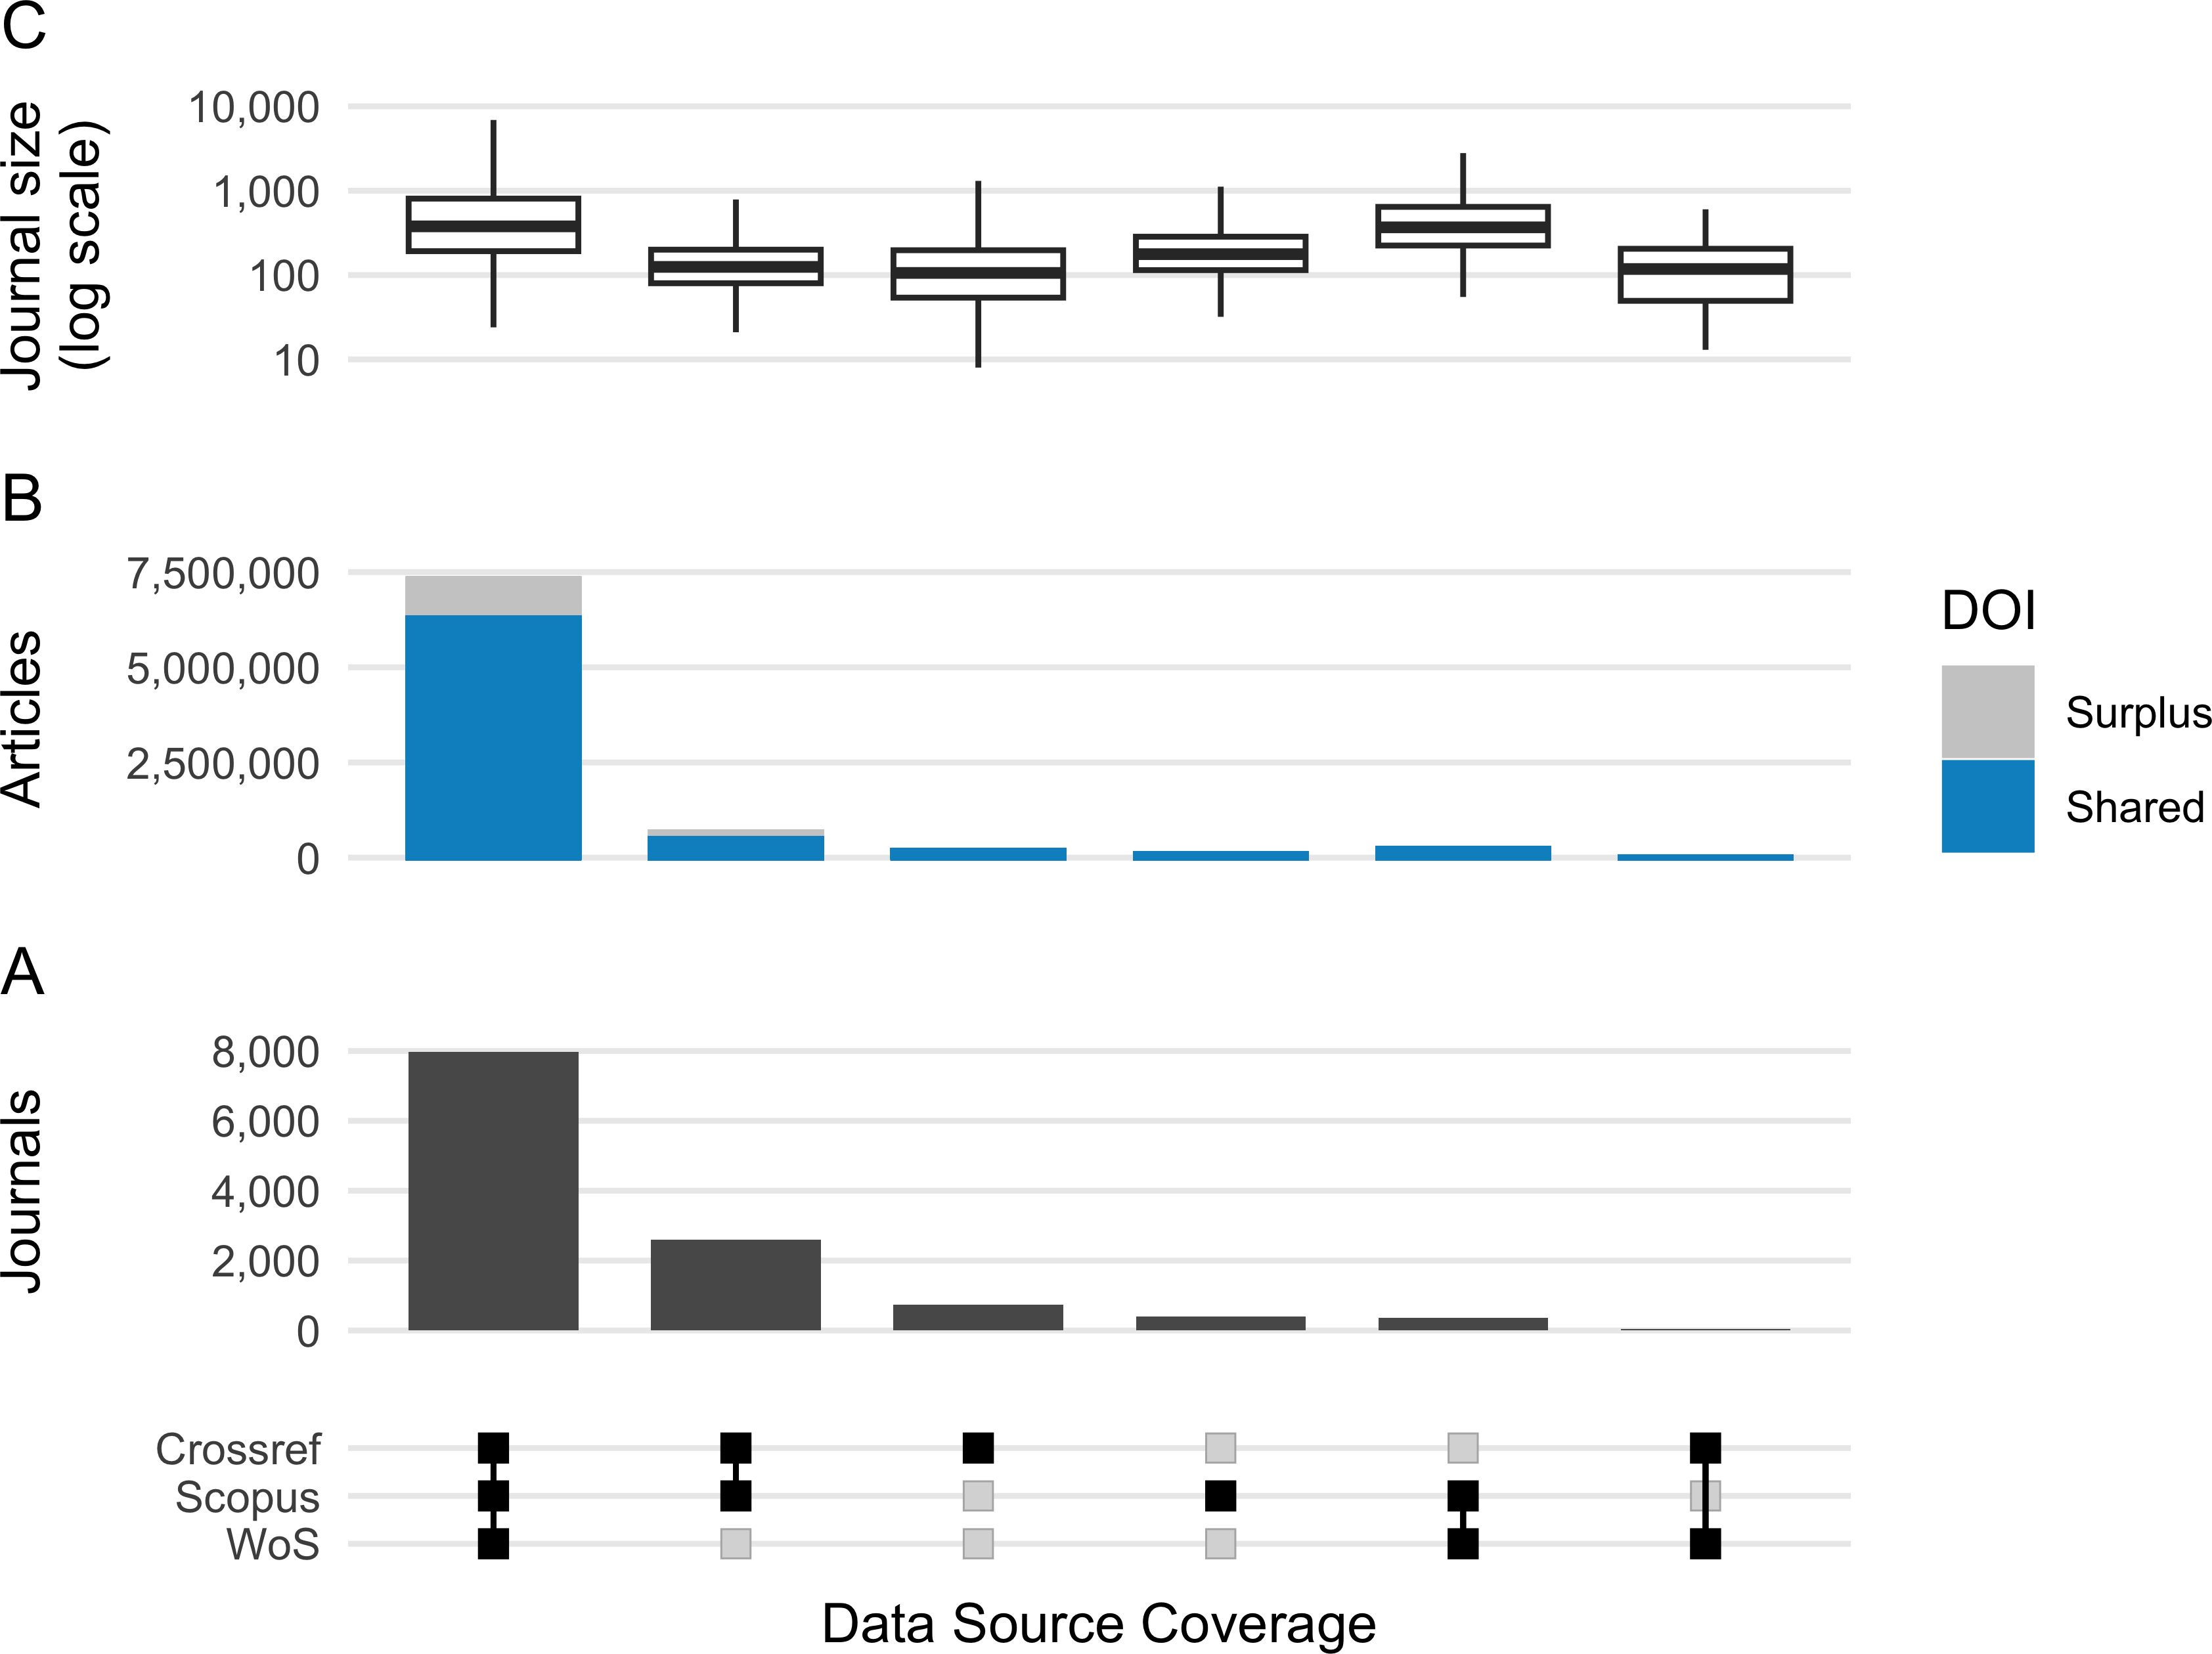
\includegraphics[width=0.99\linewidth,height=\textheight,keepaspectratio]{fig/fig-upset_coverage_results-1.png}

}

\caption{\label{fig-upset_coverage_results}Upset graph}

\end{figure}%

Journal coverage analysis revealed that 66\% (n = 7,970) of hybrid
journals included in transformative agreements were indexed in all three
databases ( \ref{fig-upset_coverage_results}A). The second-largest set
consisted of journals indexed in both hoaddata and Scopus, comprising
21\% (n = 2,595) of hybrid journals. Notably, 6\% (n = 739) of journals
were exclusively contained in hoaadata, while 3\% (n = 354) were only
found in the proprietory databases Scopus and Web of Science. Upon
insepction, this latter group represents hybrid journals for which no
open access evidence could be retrieved from Crossref, which serves as
the open access evidence source for hoaddata.

In terms of article coverage, Fig B shows the DOI overlap,
distinguihsing between a shared corpus and just those where a DOI was
only available through hoaddata. Upon inspection, reasons for lackign
DOI coverage in proprietory database were different publication dates
and differenc ein document type definitions. As such, demosntrates
certain uncertainies using the open approach. Overall, The majority of
articles can be found

Using DOIs also the size of journals were calculated (Fig C). It
highlights thate large spread in the intersection between all three
datasett. Journals are, on average, smaller than those just covered by
one or two sources.In particular journals exlcusively covered by
hoaddata are significant smaller than those covered by all three
sources.

This study compares results drawn from the openly available and
regularly updated hoaddata, an R package leveraging the open scholarly
data sources Crossref and OpenAlex, with the in-house database of the
German Competence Network Overall, xxxx hybrid journals included in xxx
agreements that published at least one open access article between 2019
and 2023.

\section*{discussion}\label{discussion}
\addcontentsline{toc}{section}{discussion}

\phantomsection\label{refs}
\begin{CSLReferences}{1}{0}
\bibitem[\citeproctext]{ref-Baas_2020}
Baas, J., Schotten, M., Plume, A., Côté, G., \& Karimi, R. (2020).
Scopus as a curated, high-quality bibliometric data source for academic
research in quantitative science studies. \emph{Quantitative Science
Studies}, \emph{1}(1), 377--386.
\url{https://doi.org/10.1162/qss_a_00019}

\bibitem[\citeproctext]{ref-Birkle_2020}
Birkle, C., Pendlebury, D. A., Schnell, J., \& Adams, J. (2020). Web of
science as a data source for research on scientific and scholarly
activity. \emph{Quantitative Science Studies}, \emph{1}(1), 363--376.
\url{https://doi.org/10.1162/qss_a_00018}

\bibitem[\citeproctext]{ref-van_Eck_2022}
Eck, N. J. van, \& Waltman, L. (2022). \emph{Crossref as a source of
open bibliographic metadata}.
\url{https://doi.org/10.31222/osf.io/smxe5}

\bibitem[\citeproctext]{ref-Geschuhn_2017}
Geschuhn, K., \& Stone, G. (2017). It's the workflows, stupid! What is
required to make {``offsetting''} work for the open access transition.
\emph{Insights the {UKSG} Journal}, \emph{30}(3), 103--114.
\url{https://doi.org/10.1629/uksg.391}

\bibitem[\citeproctext]{ref-Haupka_2024}
Haupka, N., Culbert, J. H., Schniedermann, A., Jahn, N., \& Mayr, P.
(2024). \emph{Analysis of the publication and document types in
OpenAlex, web of science, scopus, pubmed and semantic scholar}. arXiv.
\url{https://doi.org/10.48550/ARXIV.2406.15154}

\bibitem[\citeproctext]{ref-Jahn_2025}
Jahn, N. (2025). How open are hybrid journals included in transformative
agreements? \emph{Quantitative Science Studies}, 1--39.
\url{https://doi.org/10.1162/qss_a_00348}

\bibitem[\citeproctext]{ref-ComplexUpset}
Krassowski, M. (2020). \emph{ComplexUpset}.
\url{https://doi.org/10.5281/zenodo.3700590}

\bibitem[\citeproctext]{ref-Lex_2014}
Lex, A., Gehlenborg, N., Strobelt, H., Vuillemot, R., \& Pfister, H.
(2014). UpSet: Visualization of intersecting sets. \emph{IEEE
Transactions on Visualization and Computer Graphics}, \emph{20}(12),
1983--1992. \url{https://doi.org/10.1109/tvcg.2014.2346248}

\bibitem[\citeproctext]{ref-Marwick_2018}
Marwick, B., Boettiger, C., \& Mullen, L. (2018). Packaging data
analytical work reproducibly using {R} (and friends). \emph{The American
Statistician}, \emph{72}(1), 80--88.
\url{https://doi.org/10.1080/00031305.2017.1375986}

\bibitem[\citeproctext]{ref-Melero_Fuentes_2025}
Melero-Fuentes, D., Aguilar-Moya, R., Valderrama-Zurián, J.-C., \&
Gorraiz, J. (2025). Evolution and effect of meeting abstracts in JCR
journals. \emph{Journal of Informetrics}, \emph{19}(1), 101631.
\url{https://doi.org/10.1016/j.joi.2024.101631}

\bibitem[\citeproctext]{ref-Piwowar_2018}
Piwowar, H., Priem, J., Larivière, V., Alperin, J. P., Matthias, L.,
Norlander, B., Farley, A., West, J., \& Haustein, S. (2018). The state
of {OA}: A large-scale analysis of the prevalence and impact of open
access articles. \emph{{PeerJ}}, \emph{6}, e4375.
\url{https://doi.org/10.7717/peerj.4375}

\bibitem[\citeproctext]{ref-schmidt_2024_13935407}
Schmidt, M., Rimmert, C., Stephen, D., Lenke, C., Donner, P., Gärtner,
S., Taubert, N., Bausenwein, T., \& Stahlschmidt, S. (2024). \emph{The
data infrastructure of the {German Kompetenznetzwerk Bibliometrie}: An
enabling intermediary between raw data and analysis}. Zenodo.
\url{https://doi.org/10.5281/zenodo.13935407}

\bibitem[\citeproctext]{ref-Singh_2021}
Singh, V. K., Singh, P., Karmakar, M., Leta, J., \& Mayr, P. (2021). The
journal coverage of web of science, scopus and dimensions: A comparative
analysis. \emph{Scientometrics}, \emph{126}(6), 5113--5142.
\url{https://doi.org/10.1007/s11192-021-03948-5}

\bibitem[\citeproctext]{ref-Visser_2021}
Visser, M., Eck, N. J. van, \& Waltman, L. (2021). Large-scale
comparison of bibliographic data sources: {Scopus, Web of Science,
Dimensions, Crossref, and Microsoft Academic}. \emph{Quantitative
Science Studies}, \emph{2}(1), 20--41.
\url{https://doi.org/10.1162/qss_a_00112}

\end{CSLReferences}

\end{document}
